% !TEX program = pdflatex
\documentclass[10pt,twocolumn]{article}

\usepackage[margin=0.85in]{geometry}
\usepackage{amsmath,amssymb,amsfonts}
\usepackage{booktabs}
\usepackage{enumitem}
\usepackage{hyperref}
\usepackage{xcolor}
\usepackage{graphicx}
\usepackage{float}
\usepackage{cuted}
\usepackage{multirow}
\usepackage{array}
\usepackage[T1]{fontenc}
\usepackage{lmodern}
\usepackage{microtype}
% \usepackage{algorithm}
% \usepackage{algpseudocode}
\usepackage{bm}
\usepackage{tikz}
\usetikzlibrary{arrows.meta, positioning, fit, backgrounds, calc}
\usepackage{caption}
\usepackage{subcaption}
\usepackage[numbers,sort&compress]{natbib}
\usepackage[skip=4pt plus 0pt,indent=0pt]{parskip}

\usepackage{titlesec}

\titlespacing*{\section}{0pt}{8pt}{8pt}
\titlespacing*{\subsection}{0pt}{8pt}{8pt}
\titlespacing*{\paragraph}{0pt}{4pt}{0.75em}

% Compact lists
\setlist{leftmargin=*}

\hypersetup{colorlinks=true,linkcolor=blue!60!black,citecolor=green!50!black,urlcolor=blue!70!black}

% Shorthand
\newcommand{\R}{\mathbb{R}}
\newcommand{\E}{\mathbb{E}}
\newcommand{\Var}{\mathrm{Var}}
\DeclareMathOperator*{\argmin}{arg\,min}
\DeclareMathOperator*{\argmax}{arg\,max}
\newcommand{\clip}{\mathrm{clip}}

\title{%
  Toward Visually Robust Quadruped Parkour\\
  via Monocular Depth Estimation
}
\author{
  Theo Lemay \\
  \textit{Undergraduate Thesis} \\
  \texttt{theo.lemay@queensu.ca}
}
\date{April 2026}

\begin{document}
\maketitle

\begin{abstract}
  Vision-based quadruped parkour typically relies on onboard depth cameras, limiting deployment to robots with specialized sensors. We investigate whether a pre-trained \emph{monocular depth estimator} can replace depth cameras for locomotion by producing a canonical depth representation from RGB, without photorealistic rendering or domain randomization.

  We present a two-stage pipeline: a privileged teacher trained via PPO with ground-truth terrain scans, distilled into a visual student via DAgger operating on depth images from Depth~Anything~V2 (DA2). In simulation, this pipeline enables basic parkour on stairs, hurdles, and gaps under conditions characterized by a \emph{Depth Signal Quality} (DSQ) metric. Visual robustness experiments show that DA2-based students tolerate moderate lighting and color perturbations within simulation, though performance degrades on featureless surfaces and under combined perturbations. All results are in simulation; real-world transfer remains future work.
\end{abstract}

\section{Introduction}
\label{sec:intro}
% ====================================================================

Legged robots that traverse irregular terrain---stairs, hurdles, gaps---must perceive geometry and maintain tight coordination between vision and control.
Training locomotion policies in simulation with reinforcement learning (RL) and transferring them to real hardware has proven effective for agile skills~\citep{hwangbo2019learning, lee2020learning, rudin2022learning}, and recent work~\citep{zhuang2023robot, cheng2023parkour, hoeller2024anymal, chane2025soloparkour} has extended this to parkour---climbing, jumping, and crawling---via teacher--student distillation.
In these systems, a \emph{teacher} trains with privileged terrain information (e.g.\ ground-truth heightmaps), then a \emph{student} reproduces the teacher's behavior from onboard sensors.

A critical assumption, however, is access to an onboard depth sensor.
Depth cameras (e.g.\ Intel RealSense) transfer well from simulation~\citep{miki2022learning, agarwal2023legged}, but not all platforms include them---the Unitree Go2, for instance, ships with only RGB cameras and a LiDAR sensor, with no onboard depth camera~\citep{unitreego2}.

Deploying RGB-trained policies on real robots requires bridging the \emph{sim-to-real gap}.
Three strategies have emerged: (1)~\textbf{domain randomization}~\citep{tobin2017domain}, which randomizes visual properties; (2)~\textbf{generative augmentation}~\citep{yu2024lucidsim}, which uses diffusion models for photorealistic training images; and (3)~\textbf{canonical representations}, which project both domains into a shared space via a foundation model.

We pursue strategy~(3) using Depth~Anything~V2 (DA2)~\citep{yang2024depth}, a pre-trained monocular depth estimator trained on millions of diverse real images.
We propose that because DA2 maps arbitrary RGB to a depth space that is
largely robust to appearance variation, a student policy operating on
estimated depth may inherit that robustness without photorealistic
rendering or explicit domain randomization.

\paragraph{Thesis statement.}
We hypothesize that pre-trained monocular depth estimation can serve as a
visually robust intermediate representation for vision-based quadruped
parkour, allowing a student trained on estimated depth in simulation to
generalize across visual domains.
We evaluate this hypothesis entirely in simulation; real-world transfer
remains future work.

\paragraph{Contributions.}
\begin{itemize}[nosep,leftmargin=*]
  \item A two-stage teacher--student pipeline from privileged scandot
    heightmaps to monocular depth for quadruped parkour.
  \item A demonstration that monocular depth enables basic parkour (stairs, hurdles, gaps) in simulation.
  \item Identification of depth signal quality---governed by
    model scale and terrain texture---as the key factor limiting performance.
  \item A domain invariance experiment testing DA2-based students under visual perturbations.
\end{itemize}

\section{Related Work}
\label{sec:related}
% ====================================================================

\paragraph{RL for legged locomotion.}
Modern quadruped controllers are typically learned via reinforcement
learning in simulation and transferred to real
hardware~\citep{hwangbo2019learning, rudin2022learning}.
\citet{chen2020learning} introduced the privileged
teacher--student paradigm, where a teacher with access to ground-truth
simulator state is distilled into a sensorimotor student.
\citet{lee2020learning} applied it to locomotion, training a student
from proprioceptive history alone and achieving sim-to-real
transfer on rough terrain.
\citet{kumar2021rma} introduced rapid motor adaptation, using a
learned module to estimate privileged parameters online.
\citet{miki2022learning} extended the framework to perceptive
locomotion with exteroceptive depth inputs.

\paragraph{Vision-based parkour.}
\citet{agarwal2023legged} introduced the scandot
representation for depth-based locomotion, distilling a
privileged teacher into a visual student.
Extreme Parkour~\citep{cheng2023parkour} and Robot Parkour
Learning~\citep{zhuang2023robot} build on this with CNN--GRU students
that process depth images, demonstrating climbing, jumping, and
crawling on real quadrupeds.
SoloParkour~\citep{chane2025soloparkour} replaces distillation with
off-policy RL warm-started from privileged experience, and
ANYmal Parkour~\citep{hoeller2024anymal} uses a hierarchical
skill-selection policy.
All five systems assume access to a depth camera at deployment.

\citet{jenkins2024learning} is the closest work to ours,
training an RGB parkour policy using visual domain randomization with a
fine-tuned MobileNetV2 backbone. In real-world trials, Jenkins
succeeded on hurdles but failed on gaps, suggesting that domain
randomization alone may not fully close the visual sim-to-real gap.

\paragraph{Sim-to-real for vision.}
Domain randomization~\citep{tobin2017domain} perturbs visual properties
(textures, lighting, colors) so the policy learns invariance through
exposure.
LucidSim~\citep{yu2024lucidsim} replaces randomization with
generative models that produce photorealistic training images.
\citet{xue2025opening} also uses photorealistic simulation for humanoid
loco-manipulation from RGB.
All three approaches require substantial rendering overhead.

\paragraph{Monocular depth estimation.}
MiDaS~\citep{ranftl2020towards} pioneered monocular
depth estimation.
Depth~Anything~V2 (DA2)~\citep{yang2024depth} achieves state-of-the-art
depth estimation using a vision transformer encoder trained
on 142M images, able to predict depth in meters.
Figure~\ref{fig:da2_qualitative}
shows example outputs.

\begin{figure}[htbp]
	\centering
	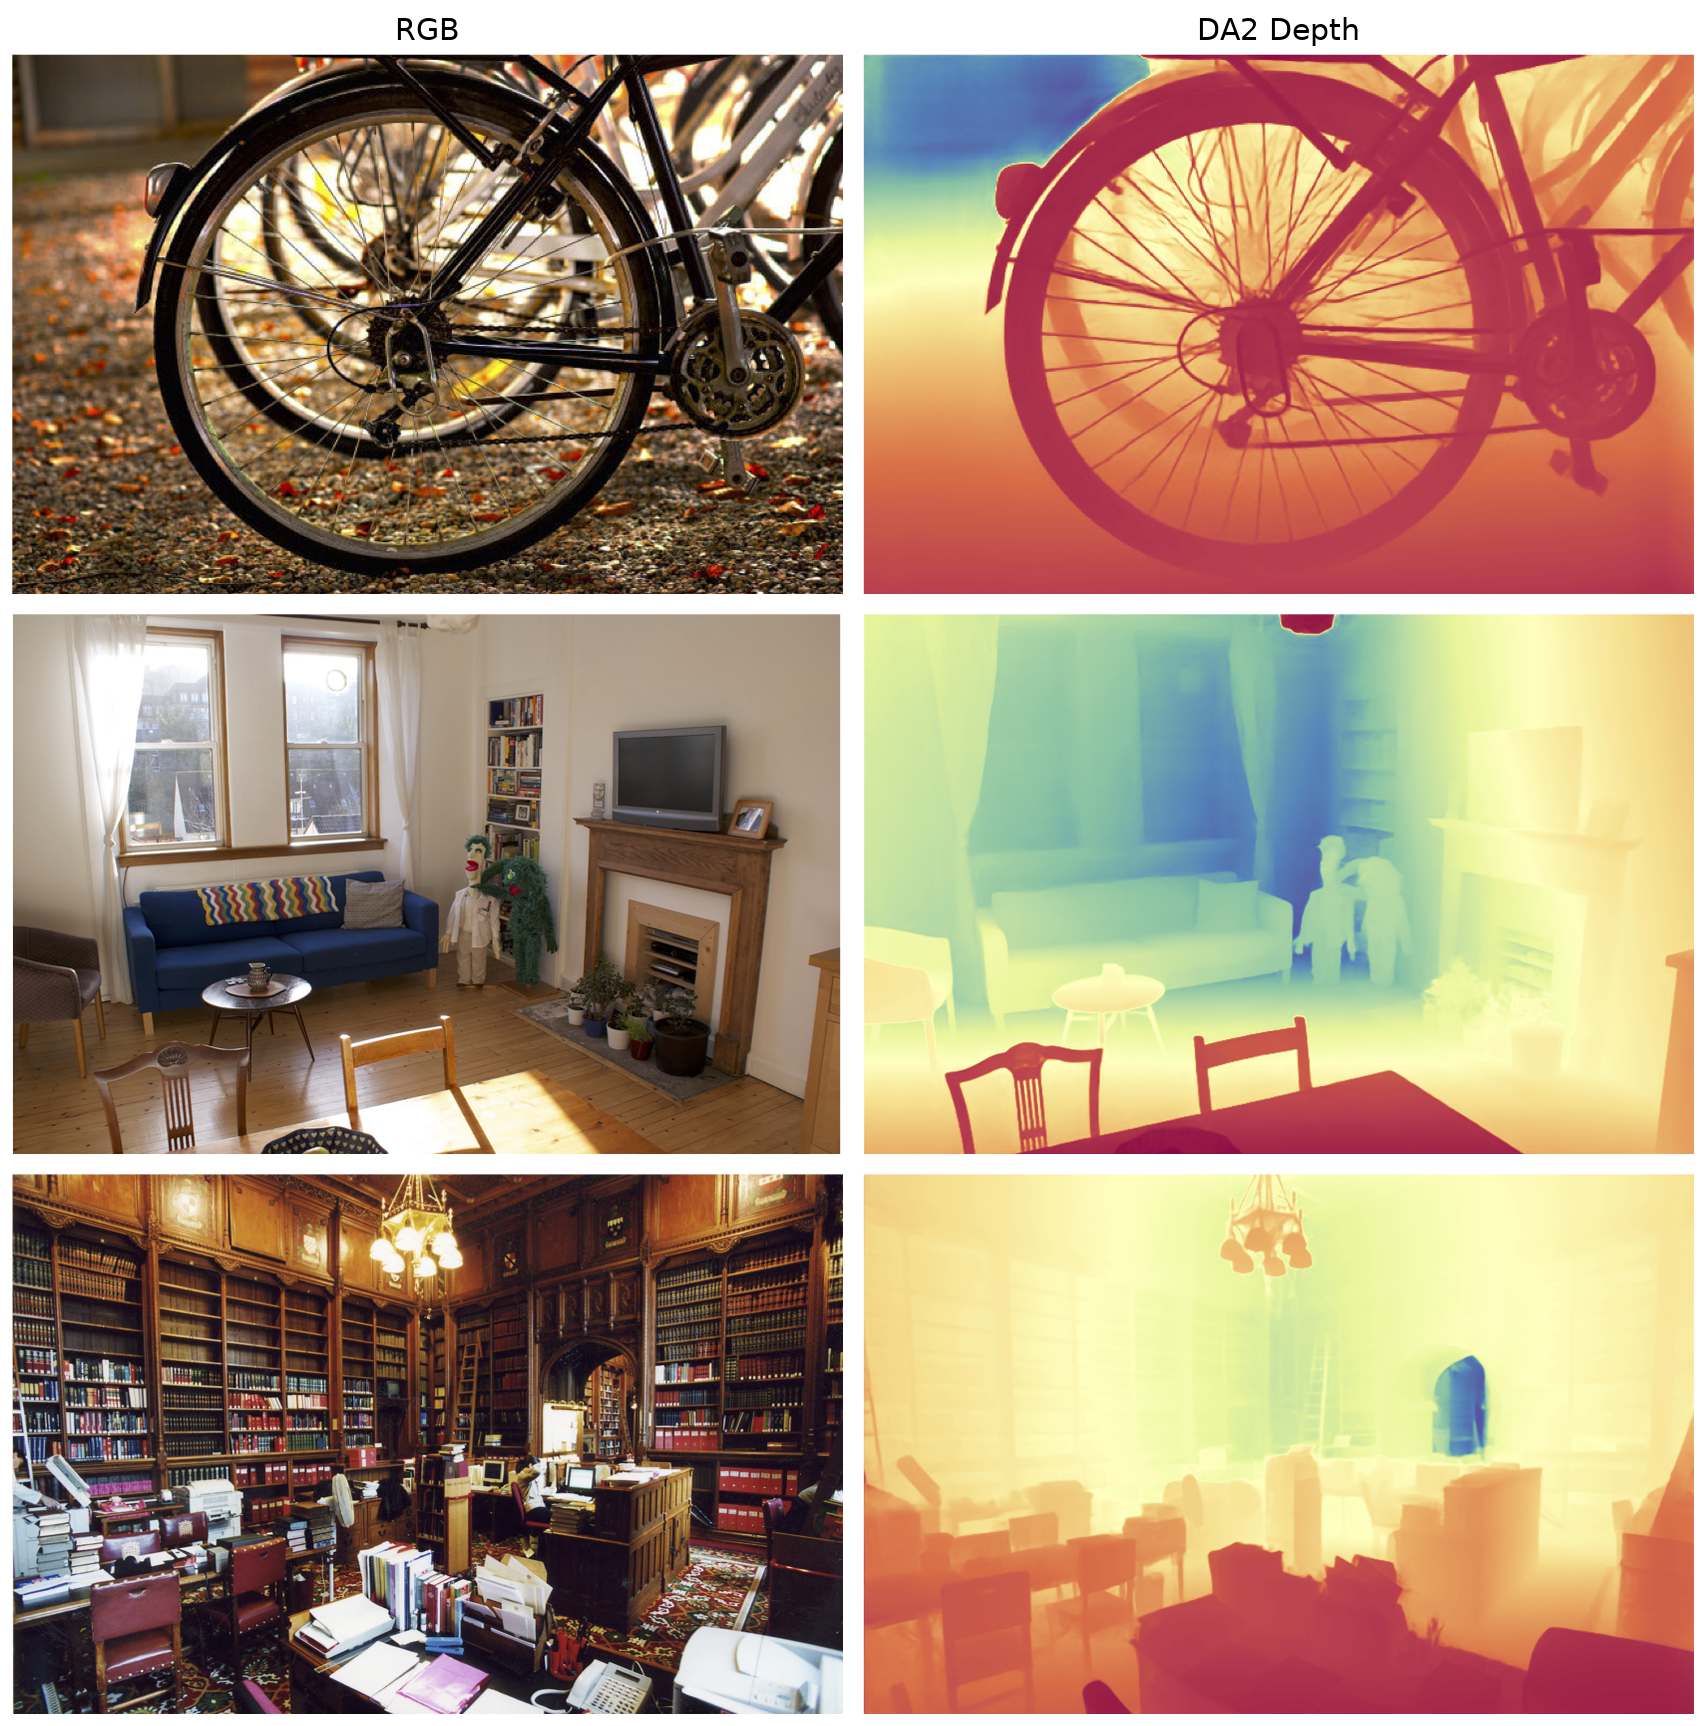
\includegraphics[width=\linewidth]{figures/depth_anything_v2_demo.png}
	\caption{Depth Anything V2 \cite{yang2024depth,depthanythingv2repo}.}
	\label{fig:da2_qualitative}
\end{figure}

\section{Mathematical Foundations}
\label{sec:math}
% ====================================================================

\subsection{Problem Formulation}

We model the parkour task as a Partially Observable Markov Decision
Process (POMDP) $(\mathcal{S}, \mathcal{A}, \mathcal{O}, T, R, \gamma)$
with state space $\mathcal{S}$, action space $\mathcal{A}$,
observation space $\mathcal{O}$, transition dynamics
$T(s'\mid s,a)$, reward $R(s,a)$, and discount factor $\gamma \in [0,1)$.

The agent receives partial observation $o_t \in \mathcal{O}$
and selects target joint position offsets
$a_t \in \mathcal{A} = \R^{12}$.
Observations decompose into:
\begin{itemize}
	\item \textbf{Proprioception} $o_\text{prop} \in \R^{53}$: base
	      angular velocity, projected gravity, velocity and heading
	      commands, joint positions, joint velocities, previous
	      actions, and foot contacts.
	\item \textbf{Exteroception} $o_\text{ext}$: scandot
	      heightmaps ($\R^{132}$) for the teacher, or depth images
	      for the student.  Scandots~\citep{agarwal2023legged} sample terrain
	      height on a $12 \times 11$ grid in the robot's body frame,
	      recording the height difference between the base and the
	      surface, clipped to $[-1, 1]$.
\end{itemize}

The objective is to find a policy $\pi$ maximizing the expected
discounted return
$J(\pi) = \E_\pi\!\left[\sum_{t=0}^{\infty} \gamma^t R(s_t, a_t)\right]$.
In a POMDP, the optimal policy generally depends on the full belief
state.  In practice, we approximate this with a recurrent architecture
(Section~\ref{sec:student}) that integrates observations over time.

\subsection{PPO}
\label{sec:ppo}

The teacher policy $\pi_\theta$ is trained with Proximal Policy
Optimization (PPO)~\citep{schulman2017proximal}.
Policy gradient methods optimize $J(\pi_\theta)$ by estimating
$\nabla_\theta J$ from trajectory samples, but naively updating
$\theta$ with large steps can collapse performance.
Trust Region Policy Optimization (TRPO)~\citep{schulman2015trust}
constrains the KL divergence between successive policies; PPO
approximates this constraint with a clipped surrogate:
\begin{equation}
	L^{\text{CLIP}} = \E_t\!\left[\min\!\left(
		r_t \hat{A}_t,\;
		\clip(r_t, 1{-}\epsilon, 1{+}\epsilon)\,\hat{A}_t
		\right)\right],
	\label{eq:ppo}
\end{equation}
where $r_t = \pi_\theta(a_t|o_t) / \pi_{\theta_{\text{old}}}(a_t|o_t)$
is the probability ratio.
The advantage estimate $\hat{A}_t$ controls the effect of the gradient.  GAE~\citep{schulman2016high} defines
\begin{equation}
	\hat{A}_t^{\text{GAE}(\gamma,\lambda)}
	= \sum_{l=0}^{\infty} (\gamma\lambda)^l \,\delta_{t+l},
	\quad
	\delta_t = r_t + \gamma V(s_{t+1}) - V(s_t),
	\label{eq:gae}
\end{equation}
where $\delta_t$ is the one-step residual and $\lambda\in[0,1]$.

When $\hat{A}_t > 0$ the clip prevents $r_t$ from exceeding
$1+\epsilon$; when $\hat{A}_t < 0$ it prevents $r_t$ from dropping
below $1-\epsilon$.


The teacher's reward combines task progress with locomotion
regularization. Table~\ref{tab:reward} lists all terms and scales.

\subsection{DAgger Distillation}
\label{sec:dagger}

The student is trained via Dataset Aggregation
(DAgger)~\citep{ross2011reduction}.  Behavioral cloning on a fixed
expert dataset suffers error compounding, but DAgger reduces this by iteratively
collecting data under the student's own distribution while labeling
with the expert.  The student observes $o_\text{prop}$ and a depth
image and predicts $a_\text{student}$, but the teacher's action
$a_\text{teacher}$ is executed.  The loss is:
\begin{equation}
	\mathcal{L} =
	\underbrace{\|a_\text{teacher} - a_\text{student}\|_2}_{\text{action loss}}
	+ \underbrace{\|y_\text{oracle} - \hat{y}\|_2}_{\text{yaw loss}},
	\label{eq:dagger_loss}
\end{equation}
where $\hat{y} \in \R^2$ is the student's predicted heading and
$y_\text{oracle}$ is ground truth heading.

\subsection{Monocular Depth Estimation}
\label{sec:depth_math}

Recovering depth from a single RGB image is an ill-posed problem:
infinitely many 3D scenes can produce the same 2D projection.
Monocular depth estimators resolve this ambiguity by learning
geometric priors from large-scale data.  Given an image
$I \in \R^{H \times W \times 3}$, the model predicts a depth map
$\hat{d} = f_\phi(I) \in \R^{H \times W}$.

\subsection{Depth Signal Quality}
\label{sec:dsq_math}

To measure how well the estimated depth preserves terrain geometry,
we define Depth Signal Quality (DSQ) as the Pearson correlation
between ground-truth and estimated depth, averaged over environments
and time:
\begin{equation}
	\mathrm{DSQ} = \frac{1}{T} \sum_{t=1}^{T}
	\frac{1}{N} \sum_{i=1}^{N}
	\rho(d^{\mathrm{GT}}_i,\, d^{\mathrm{DA2}}_i),
	\label{eq:dsq}
\end{equation}
where $\rho(\cdot,\cdot)$ denotes the Pearson correlation computed
over all pixels $p$ within each frame.

Pearson correlation is invariant to affine transformations of either
argument, i.e. $\rho(\alpha x + \beta,\, y) = \rho(x, y)$ for any
$\alpha > 0$.  This makes DSQ insensitive to the scale--shift
ambiguity inherent in monocular depth.

\section{System Architecture}
\label{sec:arch}
% ====================================================================

\subsection{Overview}

All experiments use the Genesis GPU
simulator~\cite{genesis2024} with the
legged\_gym framework~\cite{rudin2022learning} and
rsl\_rl~\cite{schwarke2025rslrl} on 4$\times$ NVIDIA L40S GPUs.
The robot is a Unitree Go2 quadruped with 12 actuated joints.
Actions $a_t \in \R^{12}$ are target joint positions, updated at 50Hz and converted to torques via a PD controller.
\begin{equation}
  \tau = K_p (a_t - q) - K_d \dot{q},
  \label{eq:pd}
\end{equation} 

The system follows the two-stage privileged distillation pipeline
described in Section~\ref{sec:intro}: a teacher trains with
ground-truth scandot heightmaps~\cite{agarwal2023legged}, then a
student reproduces the teacher's behavior from depth or RGB images
via DAgger (Figure~\ref{fig:pipeline}).

\begin{figure}[t]
  \centering
  % \includegraphics[width=\columnwidth]{figures/pipeline.pdf}
  \fbox{\parbox[c][4.5em][c]{0.9\columnwidth}{\centering
      \textbf{[Pipeline diagram]}\\
      Teacher (scandots) $\to$ Student (depth/RGB)}}
  \caption{Two-stage training pipeline.  The teacher uses privileged
    scandot observations; the student replaces these with either GT depth,
  DA2-inferred depth.}
  \label{fig:pipeline}
\end{figure}

\subsection{Teacher}

The teacher policy $\pi_T$ maps proprioception, privileged physics
parameters, and scandot heightmaps to joint targets.  Three parallel
MLPs encode each observation group into 32-dim latent vectors, which
are concatenated with proprioception and fed through the actor MLP
$\R^{n} \to \R^{12}$ to produce joint position offsets. 

\subsection{Student}
\label{sec:student}

The student replaces the scandot encoder with a visual encoder that
must recover the terrain latent $z \in \R^{32}$ from a depth image (Figure~\ref{fig:student_arch}).
A CNN maps the depth image $d \in \R^{58 \times 87}$ to a 32-dim
feature, which is concatenated with proprioception and compressed by
an MLP.  A GRU integrates these fused features
across timesteps, producing $z$ and a heading estimate
$\hat{y} \in \R^{2}$.  The teacher's actor MLP is reused, taking
$[o_\text{prop};\, z]$ to output 12 joint targets.  During
DAgger distillation, the student minimizes the loss in
Eq.~\ref{eq:dagger_loss} while the teacher's actions are executed
in the environment.

\begin{figure}[t]
  \centering
  \fbox{\parbox[c][5.5em][c]{0.9\columnwidth}{\centering
      \textbf{[Student architecture diagram]}\\
      Depth CNN $\to$ Combo MLP $\to$ GRU $\to$ [latent + yaw]\\
      {}\![proprio; latent] $\to$ Actor MLP $\to$ actions}}
  \caption{Student recurrent depth encoder architecture.  The CNN
    depth backbone and proprioception feed into a GRU that produces
  a terrain latent and heading estimate.}
  \label{fig:student_arch}
\end{figure}

\subsection{Terrain and Curriculum}

The simulator generates parkour terrains with three obstacle
families (stairs, hurdles, gaps) at four difficulty levels.
Gap widths range from 0.24\,m (Row~0) to 0.50\,m (Row~3).  During
teacher training, a curriculum advances robots to harder rows upon
success.

\section{Experiments and Results}
\label{sec:experiments}
% ====================================================================

We evaluate the DA2 pipeline through three experiments:
(1)~establishing upper-bound baselines with ground-truth sensing,
(2)~closing the gap between estimated and ground-truth depth by
varying model capacity and terrain texture, and
(3)~testing domain invariance under visual perturbations.
We report \emph{success rate} (fraction of episodes completing the
full course) and \emph{progress ratio} (mean fractional distance
along the course before termination), both averaged over 256
episodes.

% ====================================================================
\subsection{Baselines}
\label{sec:baselines}

We start by establishing upper bounds for the privileged teacher and the ground-truth depth sensing student (GT-depth).
The privileged teacher achieves near-perfect success across all gap difficulties, shown in Table~\ref{tab:baselines}.

\begin{table}[h]
  \centering
  \caption{Baseline success rates on gap terrain (\%).}
  \label{tab:baselines}
  \small
  \begin{tabular}{@{}lcccc@{}}
    \toprule
    & Row~0 & Row~1 & Row~2 & Row~3 \\
    \midrule
    Scandots teacher & 98.5 & 100.0 & 99.0 & 98.5 \\
    GT-depth student & 94.5 & 94.5 & 89.1 & 87.5 \\
    Zero-depth ablation & 8.0 & 2.0 & 0.0 & 0.0 \\
    \bottomrule
  \end{tabular}
\end{table}

The GT-depth student, receiving simulator depth images,
achieves $\geq$87\% success on all rows, confirming the CNN--GRU
architecture extracts sufficient geometry from a single depth viewpoint.
A zero-depth ablation (all depth pixels set to zero)
drops success to 8\%, verifying the policy relies on depth
rather than exploiting proprioceptive heuristics.

Figure~\ref{fig:teacher_training} shows training dynamics for both
baseline stages. Reward rises steeply as the policy masters flat terrain, then continues
climbing as the adaptive curriculum exposes progressively harder
obstacles. The GT-depth student's
distillation loss drops quickly but success climbs gradually, reflecting the difficulty of recovering the
teacher's behavior from a single depth viewpoint.


\begin{figure}[h]
  \centering
  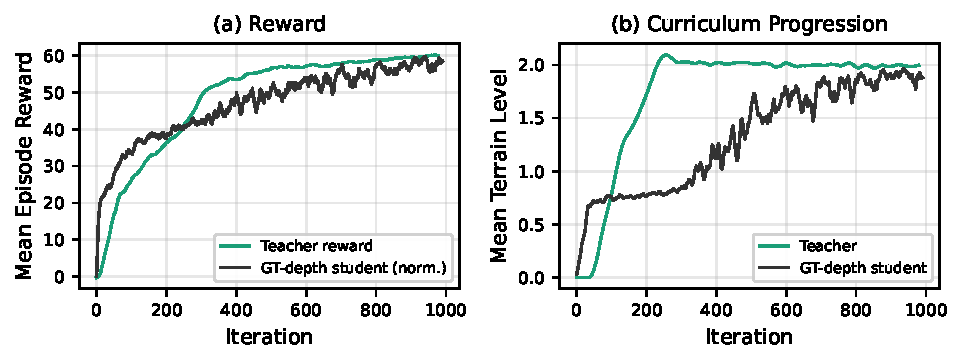
\includegraphics[width=\linewidth]{figures/teacher_training.pdf}
  \caption{Baseline training curves.}
  \label{fig:teacher_training}
\end{figure}


% ====================================================================
\subsection{Parkour from Estimated Depth}
\label{sec:da2_results}

We now determine whether parkour can be achieved from estimated
depth. Starting from the GT-depth setup, we first replace simulator
depth with DA2-small. 
As shown in Table~\ref{tab:da2_main}, 
DA2-small achieves success on Row~0 and 1, but fails completely on Rows~2 and 3.
Switching to DA2-base results in promotion to Row 3, but it still falls well short of
GT-depth on the hardest rows.

% TODO: visuals of row 1-4
% TODO: visuals of with and without texture including DA2s perception of obstacles
% TODO: depth quality metric?

The remaining limitation is the visual input. On untextured terrain,
the gap boundary provides weak monocular cues, so the depth estimate is
ambiguous. As shown in 
Table \ref{tab:da2_main},
adding checkerboard terrain texture makes the gap geometry
visible and closes most of the remaining gap to GT-depth.

Figure~\ref{fig:student_success} shows the same pattern during
training: the untextured models plateau early, while DA2-base +
texture continues improving and approaches the GT-depth student.
Breaking success down by obstacle type shows most of the gain comes from gap traversal; stairs and hurdles are much
less sensitive to texture because their geometry remains visible
without ground texture.


\begin{table}[h]
  \centering
  \caption{Policy success (\%) as model scale and terrain texture are added
  to the estimated-depth pipeline }
  \label{tab:da2_main}
  \small
  \begin{tabular}{@{}lcccc@{}}
    \toprule
    Configuration & Row~0 & Row~1 & Row~2 & Row~3 \\
    \midrule
    GT-depth baseline & 94.5 & 94.5 & 89.1 & 87.5 \\
    DA2-small & 56.3 & 33.6 & --- & --- \\
    DA2-base & 68.4 & 83.2 & 26.6 & 0.8 \\
    DA2-base + texture & 87.5 & 93.0 & 87.1 & 80.5 \\
    \bottomrule
  \end{tabular}
\end{table}

\begin{figure}[h]
  \centering
  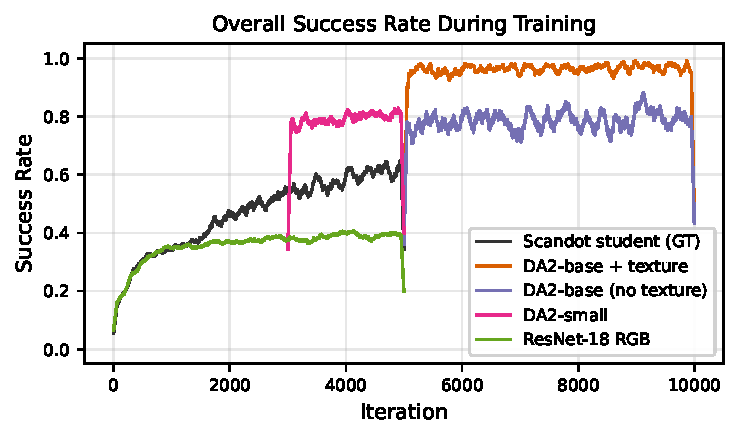
\includegraphics[width=\linewidth]{figures/student_success_comparison.pdf}
  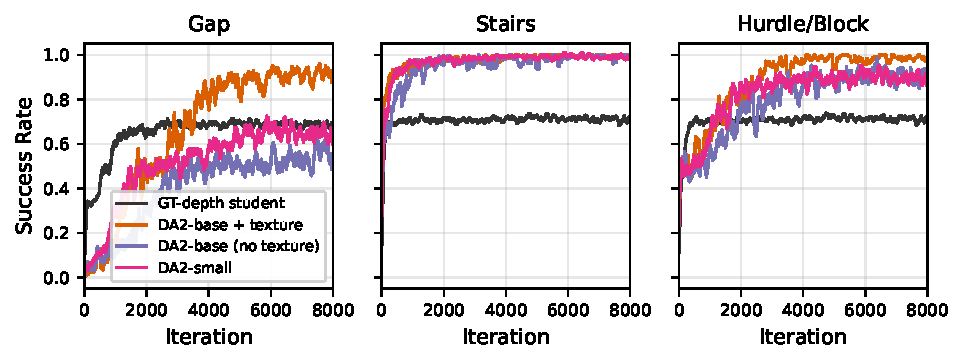
\includegraphics[width=\linewidth]{figures/per_obstacle_success.pdf}
  \caption{Overall and per-obstacle success rate during student training.}
  \label{fig:student_success}
\end{figure}

% ====================================================================
\subsection{Domain Invariance}
\label{sec:domain}

Having established strong parkour performance from estimated depth,
we now test whether DA2 provides invariance to the visual domain
shifts encountered in sim-to-real transfer. We apply perturbations
at test time only to the trained student,
covering two categories of shift: replacing the training
checkerboard with alternative surfaces, and applying brightness or per-channel color
jitter to the rendered RGB before DA2 inference.

\begin{table}[h]
  \centering
  \caption{Test-time success under visual perturbations.}
  \label{tab:domain_inv}
  \small
  \begin{tabular}{@{}p{3.6cm}rrr@{}}
    \toprule
    Perturbation & Succ. & Prog. & $\Delta$ \\
    \midrule
    Baseline (checkerboard) & 96.9\% & .948 & --- \\
    \midrule
    \multicolumn{4}{@{}l}{\textit{Texture replacement (structured)}} \\
    \quad Bricks & 89.8\% & .908 & $-$7.1 \\
    \quad Noise & 78.1\% & .843 & $-$18.8 \\
    \midrule
    \multicolumn{4}{@{}l}{\textit{Texture removal (featureless)}} \\
    \quad No texture & 18.0\% & .437 & $-$78.9 \\
    \quad Solid red & 23.4\% & .471 & $-$73.5 \\
    \quad Solid blue & 14.8\% & .417 & $-$82.1 \\
    \quad Flat grey & 18.0\% & .456 & $-$78.9 \\
    \midrule
    \multicolumn{4}{@{}l}{\textit{Color / brightness jitter}} \\
    \quad Brightness $\pm$30\% & 95.3\% & .937 & $-$1.6 \\
    \quad Brightness $\pm$60\% & 94.5\% & .935 & $-$2.4 \\
    \quad Color $\pm$15\% & 91.4\% & .914 & $-$5.5 \\
    \quad Color $\pm$30\% & 76.6\% & .816 & $-$20.3 \\
    \midrule
    \multicolumn{4}{@{}l}{\textit{Combined}} \\
    \quad Mild (bricks+b30+c15) & 82.0\% & .862 & $-$14.9 \\
    \quad Extreme (noise+b60+c30) & 63.3\% & .747 & $-$33.6 \\
    \bottomrule
  \end{tabular}
\end{table}

Table~\ref{tab:domain_inv} shows a clean separation between the two
shift types. The student is robust to the perturbations most
relevant to deployment: brightness jitter costs at most 2.4~pp,
moderate color jitter 5.5~pp, and switching to a brick texture only
7.1~pp. Performance degrades gracefully under structured noise and
combined mild perturbations, retaining 78--82\% success.

Featureless surfaces, by contrast, cause catastrophic failure
($-73$ to $-82$~pp). This is not a domain-invariance failure but a
fundamental input requirement: monocular depth estimation needs
visual features to infer geometry. Real-world surfaces (concrete,
wood, soil) all carry natural texture, so this regime is an
artifact of simulation rather than a deployment concern.

\section{Discussion and Conclusion}
\label{sec:conclusion}
% ====================================================================

\subsection{Summary}

We presented a teacher--student parkour pipeline that uses monocular
depth estimates instead of a depth camera.  The GT-depth baseline
shows that the student architecture is not the limiting factor; the
main bottleneck is depth quality.  Larger DA2 models and structured
terrain texture close most of the gap to the GT-depth baseline.

The student tolerates moderate lighting and color shifts, but fails on
featureless surfaces and some unseen textures.
DSQ is a useful indicator of whether the visual pipeline preserves
terrain structure, but it does not fully predict policy success.
Overall, monocular depth appears to be a plausible bridge from RGB to
locomotion, but actual sim-to-real transfer remains unvalidated.

\subsection{Limitations}

All experiments are in simulation, so hardware transfer is still
untested.  The task is also narrow: the obstacles are simpler than
those in recent real-world parkour systems, and the robustness study
covers only two difficulty levels.

DA2 degrades on weak-texture terrain, and DSQ does not explain every failure on unseen textures.
Because DA2 processes frames independently, its estimates may flicker.
We did not measure temporal consistency or test video-based depth
models.
Deployment would also introduce failure modes absent here, including
transparent or reflective surfaces, thin structures, motion blur, and
close-range objects near the edge of the training distribution.
Finally, the perception stack is still too heavy for onboard
deployment.  The current system is best viewed as a proof of concept.

\subsection{Future Work}

The next step is hardware evaluation on the Unitree Go2 under real
camera noise, motion blur, exposure shifts, and outdoor lighting.
Broader evaluation on harder courses would test generality.  Smaller
or temporally consistent depth models could reduce compute and
stabilize predictions, while joint adaptation of the depth estimator
and student policy may improve robustness on harder textures.



\bibliographystyle{plainnat}
\bibliography{thesis}

\newpage
\appendix
\section{Hyperparameters}
\label{sec:hyperparameters}

This appendix lists the training hyperparameters used in the
experiments.  Unless noted otherwise, values are shared across all
runs.

\subsection{Reward Function}

Table~\ref{tab:reward} lists the reward terms and scale factors used
for teacher training.  The reward at each step is
$r_t = \sum_i w_i \, r_i(s_t, a_t)$, where $w_i$ is the scale and
$r_i$ is the per-term reward signal.

\begin{table}[h]
	\centering
	\caption{Teacher reward terms and scales.}
	\label{tab:reward}
	\small
	\begin{tabular}{@{}lr@{}}
		\toprule
		Term                         & Scale                      \\
		\midrule
		\multicolumn{2}{@{}l}{\textit{Task progress}}             \\
		\quad Tracking goal velocity & 3.0                        \\
		\quad Tracking goal heading  & 1.5                        \\
		\quad Progress along course  & 2.0                        \\
		\quad Waypoint reached bonus & 20.0                       \\
		\quad Success bonus          & 40.0                       \\
		\midrule
		\multicolumn{2}{@{}l}{\textit{Termination \& collision}}  \\
		\quad Termination            & $-$50.0                    \\
		\quad Collision              & $-$2.0                     \\
		\quad Feet stumble           & $-$1.0                     \\
		\quad Feet edge              & $-$2.0                     \\
		\midrule
		\multicolumn{2}{@{}l}{\textit{Locomotion regularization}} \\
		\quad Torques                & $-$2.0$\times 10^{-4}$     \\
		\quad Joint power            & $-$2.0$\times 10^{-4}$     \\
		\quad Joint acceleration     & $-$2.0$\times 10^{-7}$     \\
		\quad Action rate            & $-$0.01                    \\
		\quad Action smoothness      & $-$0.01                    \\
		\quad Joint position limits  & $-$2.0                     \\
		\quad Torque limits          & $-$0.2                     \\
		\midrule
		\multicolumn{2}{@{}l}{\textit{Body stability}}            \\
		\quad Linear velocity $z$    & $-$0.5                     \\
		\quad Angular velocity $xy$  & $-$0.05                    \\
		\quad Orientation            & $-$0.5                     \\
		\quad Flat back              & $-$3.0                     \\
		\bottomrule
	\end{tabular}
\end{table}

\subsection{Training Hyperparameters}

PPO and DAgger training hyperparameters are listed in Tables~\ref{tab:ppo_params} and \ref{tab:dagger_params}, respectively.  Control parameters and domain randomization ranges are listed in Table~\ref{tab:control_dr}.

\begin{table}[h]
	\centering
	\caption{PPO hyperparameters for teacher training.}
	\label{tab:ppo_params}
	\small
	\begin{tabular}{@{}lr@{}}
		\toprule
		Parameter                  & Value                \\
		\midrule
		Environments               & 4096                 \\
		Steps per env per update   & 48                   \\
		Mini-batches               & 4                    \\
		Learning epochs per update & 5                    \\
		Learning rate              & $1 \times 10^{-3}$   \\
		LR schedule                & adaptive (target KL) \\
		Desired KL                 & 0.01                 \\
		Discount $\gamma$          & 0.99                 \\
		GAE $\lambda$              & 0.95                 \\
		Clip $\epsilon$            & 0.2                  \\
		Entropy coefficient        & 0.01                 \\
		Value loss coefficient     & 1.0                  \\
		Max gradient norm          & 1.0                  \\
		\bottomrule
	\end{tabular}
\end{table}


\begin{table}[h]
	\centering
	\caption{DAgger hyperparameters for student distillation.}
	\label{tab:dagger_params}
	\small
	\begin{tabular}{@{}lr@{}}
		\toprule
		Parameter                    & Value              \\
		\midrule
		Environments                 & 48                 \\
		Steps per env per update     & 120                \\
		BPTT window                  & 24                 \\
		Learning rate                & $2 \times 10^{-3}$ \\
		Actor LR scale (DA2 student) & 0.1                \\
		LR schedule (DA2 student)    & cosine             \\
		Action loss coefficient      & 1.0                \\
		Yaw loss coefficient         & 1.0                \\
		Yaw threshold (MTS)          & 0.6                \\
		Max gradient norm            & 1.0                \\
		\bottomrule
	\end{tabular}
\end{table}



\begin{table}[tbhp!]
	\centering
	\caption{PD control and domain randomization parameters.}
	\label{tab:control_dr}
	\small
	\begin{tabular}{@{}lr@{}}
		\toprule
		Parameter                    & Value                 \\
		\midrule
		\multicolumn{2}{@{}l}{\textit{PD controller}}        \\
		\quad $K_p$                  & 30.0                  \\
		\quad $K_d$                  & 0.75                  \\
		\quad Action scale           & 0.25                  \\
		\quad Control dt             & 0.02\,s (50\,Hz)      \\
		\midrule
		\multicolumn{2}{@{}l}{\textit{Domain randomization}} \\
		\quad Friction range         & [0.2, 1.7]            \\
		\quad Added base mass        & [$-$1.0, 1.0]\,kg     \\
		\quad CoM displacement $xyz$ & $\pm$0.03\,m          \\
		\quad $K_p$ / $K_d$ scale    & [0.8, 1.2]            \\
		\quad Push interval          & 15\,s                 \\
		\quad Max push velocity      & 1.0\,m/s              \\
		\bottomrule
	\end{tabular}
\end{table}



\end{document}
